%%%%%%%%%%%%%%%%%%%%%%%%%%%%%%%%%%%%%%%%%%%%%%%%%%%%%%%%%%%%%%%%
%
%  Template for homework of Introduction to Machine Learning.
%
%  Fill in your name, lecture number, lecture date and body
%  of homework as indicated below.
%
%%%%%%%%%%%%%%%%%%%%%%%%%%%%%%%%%%%%%%%%%%%%%%%%%%%%%%%%%%%%%%%%


\documentclass[11pt,letter,notitlepage]{article}
%Mise en page
\usepackage[left=2cm, right=2cm, lines=45, top=0.8in, bottom=0.7in]{geometry}
\usepackage{fancyhdr}
\usepackage{fancybox}
\usepackage{graphicx}
\usepackage{pdfpages}
\usepackage{enumitem}
\usepackage{algorithm}
\usepackage{algorithmic}
\renewcommand{\headrulewidth}{1.5pt}
\renewcommand{\footrulewidth}{1.5pt}
\newcommand\Loadedframemethod{TikZ}
\usepackage[framemethod=\Loadedframemethod]{mdframed}

\usepackage{amssymb,amsmath}
\usepackage{amsthm}
\usepackage{thmtools}
\newtheorem{lemma}{Lemma}

\setlength{\topmargin}{0pt}
\setlength{\textheight}{9in}
\setlength{\headheight}{0pt}

\setlength{\oddsidemargin}{0.25in}
\setlength{\textwidth}{6in}

\usepackage{graphicx} % more modern
\usepackage{subfigure}
\usepackage{threeparttable}

%%%%%%%%%%%%%%%%%%%%%%%%
%%%%%% Define math operator %%%%%
%%%%%%%%%%%%%%%%%%%%%%%%
\DeclareMathOperator*{\argmin}{\bf argmin}
\DeclareMathOperator*{\relint}{\bf relint\,}
\DeclareMathOperator*{\dom}{\bf dom\,}
\DeclareMathOperator*{\intp}{\bf int\,}
%%%%%%%%%%%%%%%%%%%%%%%


\setlength{\topmargin}{0pt}
\setlength{\textheight}{9in}
\setlength{\headheight}{0pt}

\setlength{\oddsidemargin}{0.25in}
\setlength{\textwidth}{6in}
\pagestyle{fancy}
%%%%%%%%%%%%%%%%%%%%%%%%
%% Define the Exercise environment %%
%%%%%%%%%%%%%%%%%%%%%%%%
\mdtheorem[
topline=false,
rightline=false,
leftline=false,
bottomline=false,
leftmargin=-10,
rightmargin=-10
]{exercise}{\textbf{Exercise}}
%%%%%%%%%%%%%%%%%%%%%%%
%% End of the Exercise environment %%
%%%%%%%%%%%%%%%%%%%%%%%


%%%%%%%%%%%%%%%%%%%%%%%%
%% Define the Problem environment %%
%%%%%%%%%%%%%%%%%%%%%%%%
\mdtheorem[
topline=false,
rightline=false,
leftline=false,
bottomline=false,
leftmargin=-10,
rightmargin=-10
]{problem}{\textbf{Problem}}
%%%%%%%%%%%%%%%%%%%%%%%
%% End of the Exercise environment %%
%%%%%%%%%%%%%%%%%%%%%%%

%%%%%%%%%%%%%%%%%%%%%%%
%% Define the Solution Environment %%
%%%%%%%%%%%%%%%%%%%%%%%
\declaretheoremstyle
[
spaceabove=0pt,
spacebelow=0pt,
headfont=\normalfont\bfseries,
notefont=\mdseries,
notebraces={(}{)},
headpunct={:\quad},
headindent={},
postheadspace={ },
postheadspace=4pt,
bodyfont=\normalfont,
qed=$\blacksquare$,
preheadhook={\begin{mdframed}[style=myframedstyle]},
	postfoothook=\end{mdframed},
]{mystyle}

\declaretheorem[style=mystyle,title=Solution,numbered=no]{solution}
\mdfdefinestyle{myframedstyle}{%
	topline=false,
	rightline=false,
	leftline=false,
	bottomline=false,
	skipabove=-6ex,
	leftmargin=-10,
	rightmargin=-10}
%%%%%%%%%%%%%%%%%%%%%%%
%% End of the Solution environment %%
%%%%%%%%%%%%%%%%%%%%%%%

%% Homework info.
\newcommand{\posted}{\text{Dec. 12, 2024}}       			%%% FILL IN POST DATE HERE
\newcommand{\due}{\text{Dec. 24, 2024}} 			%%% FILL IN Due DATE HERE
\newcommand{\hwno}{\text{6}} 		           			%%% FILL IN LECTURE NUMBER HERE


%%%%%%%%%%%%%%%%%%%%
%% Put your information here %%
%%%%%%%%%%%%%%%%%%%
\newcommand{\name}{\text{San Zhang}}  	          			%%% FILL IN YOUR NAME HERE
\newcommand{\id}{\text{PBXXXXXXXX}}		       			%%% FILL IN YOUR ID HERE
%%%%%%%%%%%%%%%%%%%%
%% End of the student's info %%
%%%%%%%%%%%%%%%%%%%


\newcommand{\proj}[2]{\textbf{P}_{#2} (#1)}
\newcommand{\lspan}[1]{\textbf{span}  (#1)  }
\newcommand{\rank}[1]{ \textbf{rank}  (#1)  }
\newcommand{\RNum}[1]{\uppercase\expandafter{\romannumeral #1\relax}}


% \lhead{
% 	\textbf{\name}
% }
% \rhead{
% 	\textbf{\id}
% }
\chead{\textbf{
		Homework \hwno
}}


\begin{document}
\vspace*{-4\baselineskip}
\thispagestyle{empty}


\begin{center}
{\bf\large Introduction to Machine Learning}\\
{Fall 2024}\\
University of Science and Technology of China
\end{center}

\noindent
Lecturer: Jie Wang  			 %%% FILL IN LECTURER HERE
\hfill
Homework \hwno             			
\\
Posted: \posted
\hfill
Due: \due
					
% \hfill

\noindent
\rule{\textwidth}{2pt}

\medskip





%%%%%%%%%%%%%%%%%%%%%%%%%%%%%%%%%%%%%%%%%%%%%%%%%%%%%%%%%%%%%%%%
%% BODY OF HOMEWORK GOES HERE
%%%%%%%%%%%%%%%%%%%%%%%%%%%%%%%%%%%%%%%%%%%%%%%%%%%%%%%%%%%%%%%%

\textbf{Notice, }to get the full credits, please show your solutions step by step.


\begin{exercise}[SVM for Linearly Separable Cases]
Given the training set $\mathcal{D}=\{ (\textbf{x}_i,y_i) \}_{i=1}^n$, where $\textbf{x}_i \in \mathbb{R}^d$ and $y_i \in \{ -1,1 \}$. Let
\begin{align*}
    \mathcal{D}^+=\{(\textbf{x}_i,y_i)\in\mathcal{D}:y_i=1\},\hspace{5mm}\mathcal{D}^-=\{(\textbf{x}_i,y_i)\in\mathcal{D}:y_i=-1\}.
\end{align*}
Assume that $\mathcal{D}^+$ and $\mathcal{D}^-$ are nonempty and the training set $\mathcal{D}$ is linearly separable. We have shown in Lecture 13 that SVM can be written as
\begin{align}\label{prob:SVM-1}
	&\min_{\textbf{w},b}\,\,\frac{1}{2}\| \textbf{w} \|^2, \\
	&\text{ s.t. } \min_i y_{i} ( \langle \textbf{w}, \textbf{x}_i \rangle + b ) = 1. \nonumber
\end{align}
Moreover, we further transform Problem (\ref{prob:SVM-1}) to
\begin{align}\label{prob:SVM}
    	&\min_{\textbf{w},b}\,\,\frac{1}{2}\| \textbf{w} \|^2, \\
    	&\text{ s.t. }\,\, y_{i} ( \langle \textbf{w}, \textbf{x}_i \rangle + b ) \geq 1, i=1,\ldots,n. \nonumber
\end{align}
We denote the feasible set of Problem (\ref{prob:SVM}) by $$\mathcal{F}=\{(\mathbf{w},b):y_{i} ( \langle \textbf{w}, \textbf{x}_i \rangle + b ) \geq 1, i=1,\ldots,n\}.$$

\begin{enumerate}
    \item The Euclidean distance between a linear classifier $f(\mathbf{x};\mathbf{w},b)=\langle\mathbf{w},\mathbf{x}\rangle+b$ and a point $\mathbf{z}$ is
    \begin{align*}
        d(\mathbf{z},f)=\min_{\mathbf{x}}\{\|\mathbf{z}-\mathbf{x} \|:f(\mathbf{x};\mathbf{w},b)=0\}.
    \end{align*}
    Please find the closed form of $d(\mathbf{z},f)$.
    \item Show that $\mathcal{F}$ is nonempty.
    \item Please show that Problem (\ref{prob:SVM}) admits an optimal solution.\\ (\textbf{Hint:} recall the lecture of Convex Optimization Problems)
    \item Please show that Problems (\ref{prob:SVM-1}) and (\ref{prob:SVM}) share the same set of optimal solutions.
    \item Let $(\textbf{w}^*,b^*)$ be the optimal solution to Problem (\ref{prob:SVM}). Please show that 
    
    (a) If the training set $\mathcal{D}$ is linearly separable, we have  $\mathbf{w}^*\neq0$;
    
    (b)If all samples in training set $\mathcal{D}$ are positive or negative, then $\mathbf{w}^*$ can be $0$.
    
    \item Let $(\textbf{w}^*,b^*)$ be the optimal solution to Problem (\ref{prob:SVM}). Show that there exist at least one positive sample and one negative sample, respectively, such that the corresponding equality holds. In other words, there exist $i,j \in \{ 1,2,\dots,n \}$ such that
    \begin{align*}
        1=y_i = &\langle \textbf{w}^*, \textbf{x}_i \rangle + b^*, \\
        -1=y_j = &\langle \textbf{w}^*, \textbf{x}_j \rangle + b^*.
    \end{align*}
    \item Show that the optimal solution to Problem (\ref{prob:SVM}) is unique and there is at least one of the constraints holds as an equality at the optimum.
    \item Can we remove the inequalities that hold strictly at the optimum to Problem (\ref{prob:SVM}) without affecting the solution? Please justify your claim rigorously.
    
\end{enumerate}

\end{exercise}
\begin{solution}
	
\end{solution}







\newpage
\begin{exercise}[Discussions on Geometric Multiplier and Duality Gap]
Consider the primal problem
\begin{align}\label{prob:geometric}
    \min _{\mathbf{x}}\ &f(\mathbf{x}) \\ \nonumber
    \text{s.t.}\ &g_{i}(\mathbf{x}) \leq 0,\, i=1, \cdots, m, \\ \nonumber
    &h_{i}(\mathbf{x})=0, i=1, \cdots, p, \\ \nonumber
    &\mathbf{x} \in X.
\end{align}
Recall the discussion on Geometric Multiplier and Duality Gap in Lecture 13. 
\begin{enumerate}
    \item For each of the following problems:
    \begin{enumerate}
        \item \begin{align*}
		&\min\,f(x)=x\\
		&\mbox{s.t. }g(x)=x^2\leq0,\\
		&\hspace{7mm}x\in X=\mathbb{R}.
	\end{align*}
        \item \begin{align*}
		\min\,&f(x)=
		\begin{cases}
			e^x,\,\hspace{5mm}x\leq0,\\
			1-x,\,x\in[0,1],\\
			0,\,\hspace{7mm}x>1.
		\end{cases}\\
		\mbox{s.t. }\,&g(x)=x\leq0.
	\end{align*}
        \item\begin{align*}
		\min\,&f(x)=
		\begin{cases}
			-x,\,x\leq0,\\
			0,\,\hspace{3mm}x>0.
		\end{cases}\\
		\mbox{s.t. }\,&g(x)=x\leq0.
	\end{align*}
    \end{enumerate}
    finish the following three tasks:
    \begin{enumerate}
        \item Plot the graph of $f(x)$ relative to $g(x)$, that means the horizontal axis represents $g(x)$ and the vertical axis represents $f(x)$. Refer to the Figure 1 in Lecture 13.
        \item Check whether a geometric multiplier exists and whether there is duality gap;
        \item Find the dual problem of the primal problem and try to solve the dual problem.
    \end{enumerate}

    \item Based on the above discussions, decide whether the following claims on the geometric multiplier and the duality gap for the primal problem are correct? Justify the claims rigorously if they are correct. Otherwise please give a counterexample for each.
    \begin{enumerate}
        \item The geometric multiplier for the primal problem (\ref{prob:geometric}) always exists.
        \item If the geometric multiplier exists, then it is unique.
        \item If the geometric multiplier exists, then the duality gap is zero.
        \item If the duality gap is zero, there exists at least one geometric multiplier.
        \item Let $(\lambda^*,\mu^*)$ be a geometric multiplier. Then, the problem $\argmin_{\mathbf{x}\in X} L(\mathbf{x}, \lambda^*,\mu^*)$ always admits at least one solution, where $L(\mathbf{x}, \lambda, \mu)$ is the Lagrangian for (\ref{prob:geometric}).
        \item If $(\lambda^*,\mu^*)$ is a geometric multiplier and the problem $\argmin_{\mathbf{x}\in X} L(\mathbf{x}, \lambda^*,\mu^*)$ admits a solution $\mathbf{x}^*$, then $\mathbf{x}^*$ is feasible.
        \item (optional) Let $(\lambda^*,\mu^*)$ be a geometric multiplier. Then, $\mathbf{x}^*$ is a global minimum of the primal problem if and only if $\mathbf{x}^*$ is feasible and $\mathbf{x}^*\in\argmin_{\mathbf{x}\in X}\,L(\mathbf{x},\lambda^*,\mu^*)$.
    \end{enumerate}
\end{enumerate}
\end{exercise}

\newpage

\begin{exercise}[Exercises of Dual Problems ]
    For each of the following given optimization problems with constraints, answer the following questions respectively:
    \begin{enumerate}
        \item Give the feasible set, the optimal value and the optimal solution $\mathbf{x}^*$.
        \item Write the dual problem of the primal problem, and give the KKT conditions.
        \item State whether strong duality holds for this problem and support it by precise calculation.
    \end{enumerate}
    The problems:\\
    (1)
    \begin{align*}
        \min_x\,& x^2+2x+3\\
        {\rm s.t.}\,& (x+2)(x-2)(x-4)\le 0,\\
        & (x+1)^3 \geq 1,\\
        & x\in\mathbb{R}.
    \end{align*}
    (2)
    \begin{align*}
        \min_{x_1, x_2}\,& e^{x_1}+e^{2x_2}\\
        {\rm s.t.}\,& x_1+x_2=1,\\
        & x_1, x_2\in\mathbb{R}.
    \end{align*}
\end{exercise}
\begin{solution}

\end{solution}

\newpage
\begin{exercise}[The Dual Problem of SVM]
Suppose that the training set is $\mathcal{D}=\{ (\textbf{x}_i,y_i) \}_{i=1}^n$, where $\textbf{x}_i \in \mathbb{R}^d$ and $y_i \in \{ -1,1 \}$. Let
\begin{align*}
    \mathcal{D}^+=\{(\textbf{x}_i,y_i)\in\mathcal{D}:y_i=1\},\hspace{5mm}\mathcal{D}^-=\{(\textbf{x}_i,y_i)\in\mathcal{D}:y_i=-1\}.
\end{align*}
Assume that $\mathcal{D}^+$ and $\mathcal{D}^-$ are nonempty.
The soft margin SVM takes the form of
\begin{align}\label{prob:soft-SVM-1}
    \min_{\mathbf{w},b,\boldsymbol{\xi}}\,&\frac{1}{2}\|\mathbf{w}\|^2_2+C\sum_{i=1}^n\xi_i,\\ \nonumber
    {\rm s.t.\,}&\,y_i(\langle\mathbf{w},\mathbf{x}_i\rangle+b)\geq1-\xi_i,i=1,\ldots,n,&\\ \nonumber
    &\,\xi_i\geq0,\,i=1,\ldots,n,
\end{align}
The corresponding dual problem is
\begin{align}\label{prob:dual-soft-SVM}
		\min_{\alpha}\,&\frac{1}{2}\sum_{i=1}^n\sum_{j=1}^n\,\alpha_i\alpha_jy_iy_j\langle\mathbf{x}_i,\mathbf{x}_j\rangle-\sum_{i=1}^n\alpha_i\\\nonumber
	\mbox{s.t. }\,&\sum_{i=1}^n\alpha_iy_i=0,\\\nonumber
	&\alpha_i\in[0,C],i=1,\ldots,n.
\end{align}
\begin{enumerate}
    \item Consider the relation between the primal problem and dual problem:
    \begin{enumerate}
        \item Show that the problems (\ref{prob:soft-SVM-1}) and (\ref{prob:dual-soft-SVM}) always admit optimal solutions.
        \item (Optional) For a linearly separable data sample, shall we arrive at the same separating hyperplane by solving the problems in (\ref{prob:SVM})  and (\ref{prob:dual-soft-SVM}), respectively?
    \end{enumerate}
    \item The function of the slack variables used in the optimization problem for soft margin hyperplanes takes the form $\sum_{i=1}^n \xi_i$. We could also use $\sum_{i=1}^n \xi_i^p$, where $p>1$. The soft margin SVM becomes
    \begin{align}\label{prob:soft-SVM-p}
        \min_{\mathbf{w},b,\boldsymbol{\xi}}\,&\frac{1}{2}\|\mathbf{w}\|^2_2+C\sum_{i=1}^n\xi_i^p,\\ \nonumber
        {\rm s.t.\,}&\,y_i(\langle\mathbf{w},\mathbf{x}_i\rangle+b)\geq1-\xi_i,i=1,\ldots,n,&\\ \nonumber
        &\,\xi_i\geq0,\,i=1,\ldots,n.
    \end{align}
    Please find the dual problem of (\ref{prob:soft-SVM-p}) and the corresponding optimal conditions.
    \item Let $(\mathbf{w}^*, b^*, \mathbf{\xi}^*)$ and ($\mathbf{\alpha}^*, \mathbf{\mu}^*)$ be the optimal solutions to problems (\ref{prob:soft-SVM-1}) and (\ref{prob:dual-soft-SVM}), $(\mathbf{x}_i, y_i)$ is a point from the training set. Please \textbf{give the complementary slackness conditions} of problem (\ref{prob:soft-SVM-1}) and:
    \begin{enumerate}
        \item Give the conditions that point $(\mathbf{x}_i, y_i)$ satisfies if it is a support vector.
        \item Give the conditions that point $(\mathbf{x}_i, y_i)$ satisfies if it is misclassified.
        \item Give the conditions that point $(\mathbf{x}_i, y_i)$ satisfies if it is in the region between the marginal hyperplanes.
    \end{enumerate}
    \item As shown in Figure \ref{svm}, the training set is  $\mathcal{D}=\{ (\textbf{x}_i,y_i) \}_{i=1}^{13}$, where $\textbf{x}_i \in \mathbb{R}^2$ and $y_i \in \{ +1,-1 \}$. Suppose that we use the soft margin SVM to classify the data points and get the optimal parameters $\mathbf{w}^*$, $b^*$, and $\boldsymbol{\xi}^*$  by solving the problem \eqref{prob:soft-SVM-p}.
    \begin{enumerate}
        \item Please write down the equations of the separating hyperplane ($H_0$) and the marginal hyperplanes ($H_1$ and $H_2$) in terms of $\mathbf{w}^*$ and $b^*$.
        \item Please find the support vectors and the non-support vectors.
        \item (Optional) Please find the values (or ranges) of the optimal slack variables $\xi_i^*$ for $i=1,2,\dots,13$. (\textit{Hint: The possible answers are $\xi_i^*=0$, $0<\xi_i^*<1$, $\xi_i^*=1$, and $\xi_i^*>1$}). How do the slack variables change when the parameter $C$ increases and decreases?
    \end{enumerate}
\end{enumerate}
\end{exercise}
\begin{figure}[H]
  \centering
  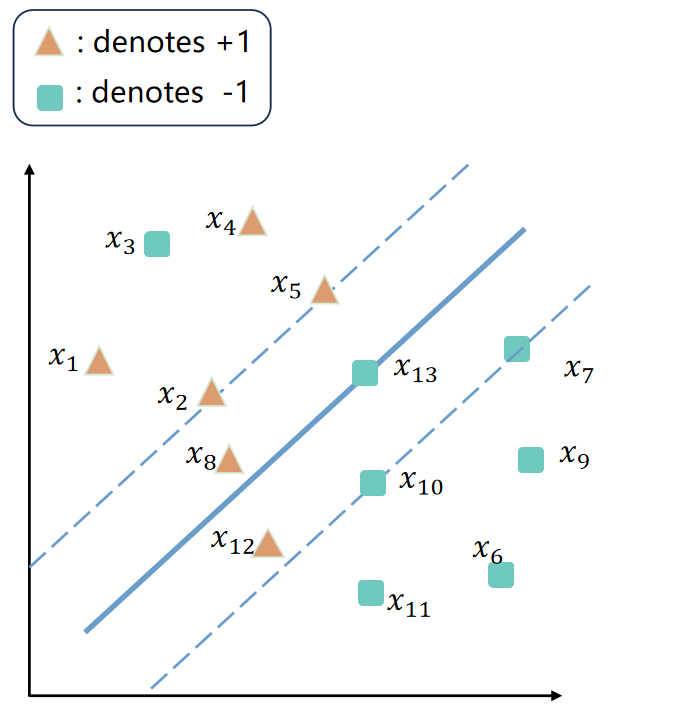
\includegraphics[width=10cm]{Figures/2024_fall_svm.png}
  \caption{Classifying the data points using the soft margin SVM. $H_0$ is the separating hyperplane. $H_1$ and $H_2$ are the marginal hyperplanes.}
  \label{svm}
\end{figure}
\begin{solution}

\end{solution}


\newpage
\begin{exercise}[Neural Networks]
\begin{enumerate}
    \item The softmax function $\textbf{f}:\mathbb{R}^n\rightarrow\mathbb{R}^n$ is defined by:
    $$f_i(\textbf{x})=\frac{\exp(x_i)}{\sum_{k=1}^{n}\exp(x_k)}, i=1,\ldots,n,$$
    where $x_i$ is the $i^{th}$ component of $\textbf{x}\in\mathbb{R}^n$. The function  $\textbf{f}(\textbf{x})=(f_1(\textbf{x}),f_2(\textbf{x}),\ldots,f_n(\textbf{x}))^{\top}$ converts each input $\textbf{x}$ into a probability (stochastic) vector in which all entries are nonnegative and add up to one.
    \begin{enumerate}
        \item Please find the gradient and Jacobian matrix of $\textbf{f}(\textbf{x})$, i.e., $\nabla \textbf{f}(\textbf{x})$ and $J\textbf{f}(\textbf{x})$.
        \item Show that $\textbf{f}(\mathbf{x})=\textbf{f}(\mathbf{x}-c\mathbf{1})$, where $c=\max\{x_1,x_2,...,x_n\}$ and $\mathbf{1}$ is a vector all of whose components are one. When do we need this transformation?
    \end{enumerate}
    \item The log softmax function is one variant of softmax function, and is defined by:
    $$f_i(\textbf{x})=\log\frac{\exp(x_i)}{\sum_{k=1}^{n}\exp(x_k)}, i=1,\ldots,n,$$
    where $x_i$ is the $i^{th}$ component of $\textbf{x}\in\mathbb{R}^n$. 
    \begin{enumerate}
        \item Please find the gradient of $\mathbf{f}(\mathbf{x})$ (definition is the same as in 1) and show that $f_i$ is concave.
        \item For classification task, the \textbf{cross entropy} is usually used as loss function and its input is the output of softmax layer. But in practice, we combine the softmax layer and cross entropy as one layer, and use log softmax function in calculation instead of softmax function. Try to clarify the advantages of log softmax function in comparison to softmax function.
    \end{enumerate}
    \item Consider the neural network with a single hidden layer in Figure 2. Let $\mathbf{x}\in\mathbb{R}^3$ be an input vector, and $\mathbf{y}$ be its corresponding output of the network. $f$ implies that there exist four units in the hidden \textbf{fully connected} layer, each of which is followed by a \textbf{sigmoid activation function} $\sigma$, converting its input $\mathbf{z}$ to output $\mathbf{a}$. Then $\mathbf{a}$ will be transformed into the output $\mathbf{y}$ through another fully connected layer. Finally we use the \textbf{softmax layer} to get the probabilities of each class and use the \textbf{entropy loss} as the loss function. Suppose that an arbitrary input vector $\mathbf{x}_0$ = $(1, 1, 1)^\top$ and its ground truth label is $[0,0,1]^\top$.
	\begin{enumerate}
            \item If we initialize the weights $W_{ij}^1 = 0.40$ where $i\in\{1,2,3,4\}$ and $j\in\{1,2,3\}$ and $W_{ij}^2 = 0.25$ where $i\in\{1,2,3\}$ and $j\in\{1,2,3,4\}$. Compute the  output $\mathbf{y}$ and loss $L$.
            \item The goal of training of this neural networks is to get the weights $\mathbf{W}^1$ and $\mathbf{W}^2$, where $\mathbf{W}^1 \in \mathbb{R}^{4\times3}$, $\mathbf{W}^2 \in \mathbb{R}^{3\times4}$. We use the \textbf{gradient decent} to learn the weights and use the \textbf{back propagation algorithm} to compute the gradient. Write the update formula  of $W_{ij}^1$ where $i\in\{1,2,3,4\}$ and $j\in\{1,2,3\}$ and $W_{ij}^2$ where $i\in\{1,2,3\}$ and $j\in\{1,2,3,4\}$ used in learning. The formula is expected to contain output $\mathbf{y}$ and ground truth $\mathbf{q}$.
            \item According to your results, try to represent them in the form of matrix. This will assist you in your project homework.
            \item Can we initialize all the parameters, i.e., weights and bias, of the neural network to zero? Please state you conclusion.\\
            (\textbf{Hint:} You can search about the initialization of weights of neural networks if interested.)
            \item Thanks to the \textbf{back propagation}, the structure of neural networks can be very flexible. Rewrite the results in (b) if we replace the \textbf{sigmoid activation function} with \textbf{relu activation function} that is 
            \begin{align*}
                \sigma(z) = \max(0, z).
            \end{align*}
	\end{enumerate}
\end{enumerate}
\end{exercise}
\begin{figure}[h]
  \centering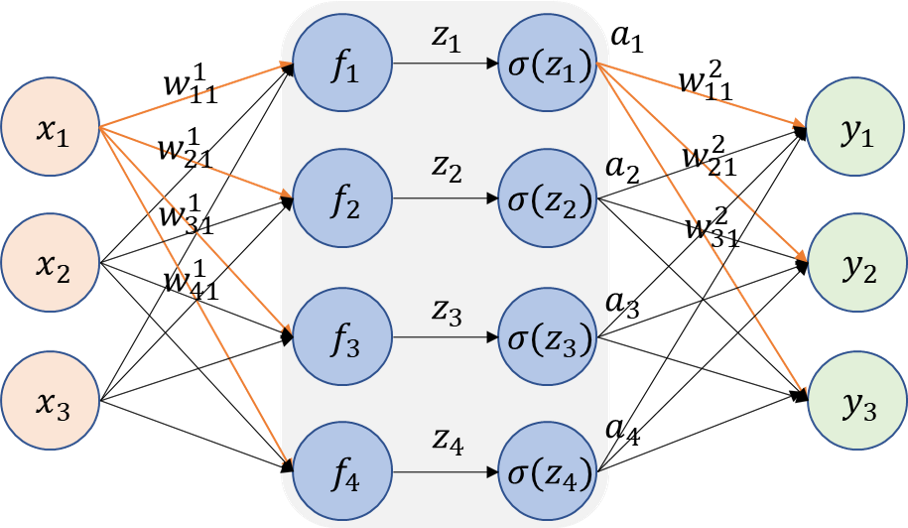
\includegraphics[width=12cm]{Figures/2021_fall_nn.png}
  \caption{A neural network with a single hidden layer.}
  \label{backpropogation}
\end{figure}
\begin{solution}${}$

\end{solution}

\newpage
\begin{exercise}[Convolutional Neural Networks and Some Advanced Networks Structure]
% \begin{exercise}[Convolutional Neural Networks]

\centering
\begin{tabular}{|c|c|c|c|c|c|c|c|}
    \hline
    conv3-32 & conv5-32 & max pool & conv3-64 & conv5-64 & max pool & FC-128 & FC-10\\
    \hline
\end{tabular}
% \caption{The architecture of convolutional neural network} \label{tab:cnn}

\begin{enumerate}
    \item Consider a convolutional neural network as shown in table above.
    \begin{enumerate}
        \item The convolutional layer parameters are denoted as ``conv$\langle$filter size$\rangle$-$\langle$number of filters$\rangle$".
        \item  The fully connected layer parameters are denoted as ``FC$\langle$number of neurons$\rangle$".
        \item The window size of pooling layers is $2$.
        \item The stride of convolutinal layers is $1$.
        \item The stride of pooling layers is $2$.
        \item You may want to use padding in both convolutional and pooling layers if necessary.
        \item For convenience, we assume that there is no activation function and bias.
    \end{enumerate}
    
    Suppose that the input is a $\mathbf{210\times 160}$ \textbf{RGB} image. Please derive the size of all feature maps and the number of parameters.
    
\end{enumerate}
\begin{enumerate}[resume]
    \item (optional) In previous discussion, the optimization method we take is actually \textbf{stochasitic}, that is we pick only one sample from the training set to compute the gradient and then update the weights. But in practice, we use \textbf{mini batch learning}, where a specific number of samples instead of only one sample or all of the samples are used to compute the loss and gradients. The loss becomes the mean of the losses of the specific number of samples. Take the cross entropy for example, the loss function becomes:
    \begin{align*}
    Loss = -\frac{1}{N}\sum_n \sum_i q_i\log (p_i),
    \end{align*}
    where $N$ is the mini batch size.\\
    The gradient $\mathbf{g}$ also becomes the mean of the gradients of the mini-batch samples:
    \begin{align*}
    \mathbf{g} = \frac{1}{N}\sum_n \mathbf{g}_n,
    \end{align*}
    where $\mathbf{g}_n$ is the computed gradient by the n$^{th}$ sample in the mini batch samples. \\
    \begin{enumerate}
        \item From perspective of computational efficiency and convergence, clarify the advantages of mini-batch.\\
        (\textbf{Hint:} Recall the discussion of convergence of mini-SGD in HW 5.)
        \item The initial values of weights and the distribution of the values will 
        greatly affect the speed of the learning. The purpose of \textbf{Batch Normalization} is to adjust the distribution of activated values of each layer. Specifically, it is to adjust the distribution of the mini batch samples to a distribution with mean equal to \textbf{0} and variance equal to \textbf{1}. \\
        For input mini batch samples $\{\mathbf{x}_1, \mathbf{x}_2, ... \mathbf{x}_m\}$, do the following tranformation:
        \begin{align*}
        &\mathbf{\mu}_B \leftarrow \frac{1}{m}\sum_{i=1}^{m} \mathbf{x}_i\\
        &\mathbf{\sigma}_B^2 \leftarrow \frac{1}{m}\sum_{i=1}^{m} (\mathbf{x}_i - \mathbf{\mu}_B)^2 \\
        &\hat{\mathbf{x}}_i \leftarrow \frac{\mathbf{x}_i - \mathbf{\mu}_B}{\sqrt{\mathbf{\sigma}_B^2 + \epsilon}}
        \end{align*}
        where $\epsilon$ is a very small number to prevent division by zero.\\
        Then output $\mathbf{y} = \{\mathbf{y}_1, \mathbf{y}_2, ... \mathbf{y}_m\}$ through an affine transformation:
        \begin{align*}
        \mathbf{y}_i \leftarrow \gamma \hat{\mathbf{x}}_i + \mathbf{\beta},
        \end{align*}
        where $\gamma$ and $\beta$ are also to be adjusted by learning. $\gamma$ is initialized with 1 and $\beta$ is initialized with 0.\\
        Compute the back propagation of \textbf{Batch Normalization Layer}.
    \end{enumerate}
\end{enumerate}

\end{exercise}

\begin{solution}
    
\end{solution}

\newpage
\begin{exercise}[Some Network Layers, Linear Transformation and Gradient ({\bf Optional})]
In this exercise, we explore several kinds of network layers in the view of linear transformation.
\begin{enumerate}
\item \textbf{1-dimensional convolutional layer.} Suppose we have an input $\mathbf{x}\in\mathbb{R}^n$ and filter $\mathbf{w}\in\mathbb{R}^k$ ($n>k$). We can compute the convolution of $\mathbf{x}\ast \mathbf{w}$ as follows:
    \begin{itemize}
      \item Take the convolutional filter $\mathbf{w}$ and align it with the beginning of $\mathbf{x}$. Take the dot product of $\mathbf{w}$ and the $\mathbf{x}[0 : k -1]$ and assign that as the first entry of the output.
      \item Suppose we have stride $s$. Shift the filter down by $s$ indices, and now take the dot product of $\mathbf{w}$ and $\textbf{x}[s : k - 1 +s]$ and assign to the next entry of your output.
      \item Repeat until we run out of entries in $\mathbf{x}$.
    \end{itemize}
    
    \begin{figure}[H]
              \centering
              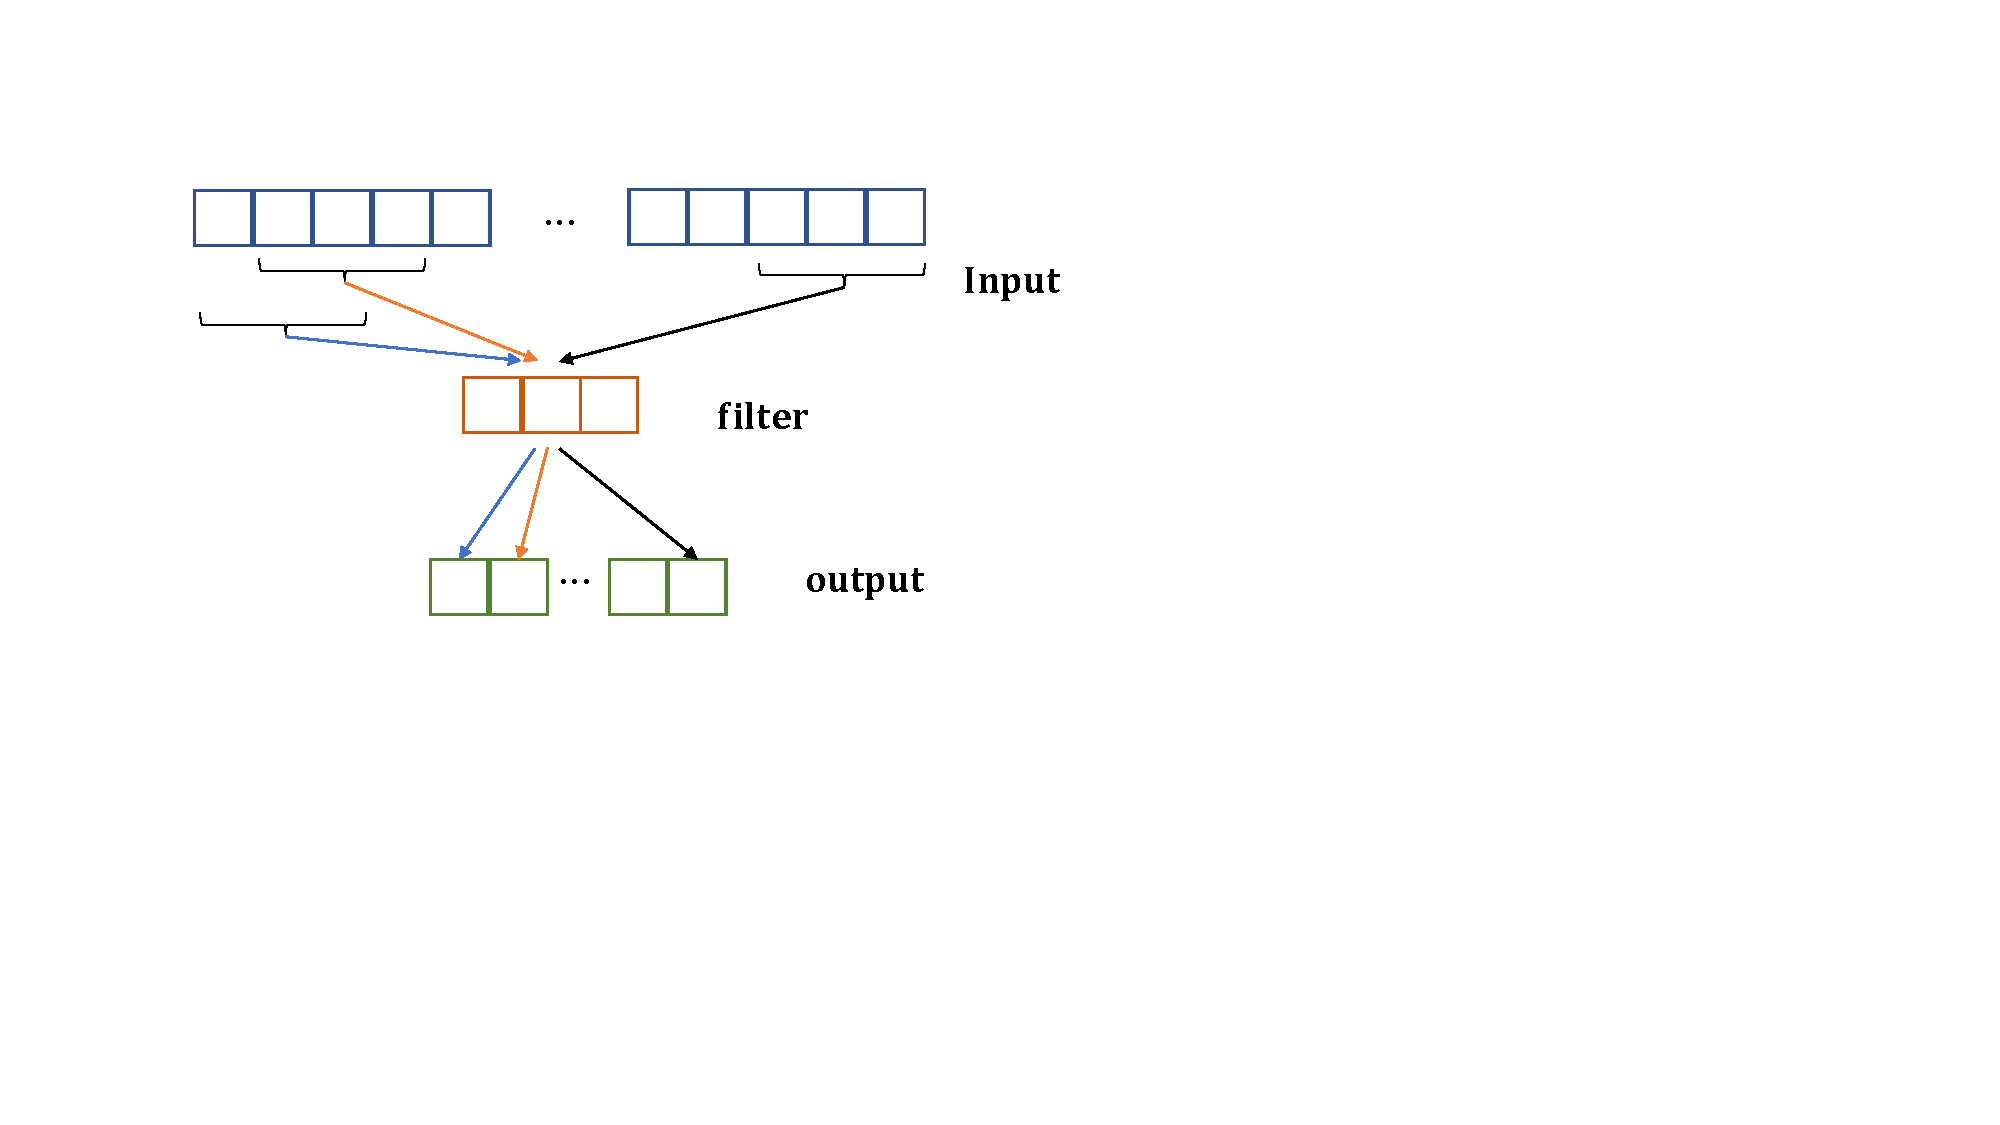
\includegraphics[width=0.6\textwidth]{Figures/1dimensioal_convolution}
              \caption{1-dimensional convolutional layer.}
            \end{figure}
    
    
    Now we set the stride $s$ to be 1:
    \begin{align*}
    \mathbf{y}=\mathbf{x}\ast \mathbf{w}=\left(\sum_{i=1}^kw_ix_i,\sum_{i=1}^kw_ix_{i+1},\cdots, \sum_{i=1}^kw_ix_{i+n-k}\right)\in\mathbb{R}^{n-k+1}.
    \end{align*}
    Is the 1-dimensional convolutional operation a linear transformation? If so, please find the transformation matrix, then write down the gradient with respective to $\mathbf{x}$.

\item \textbf{$1\times1$ convolutional layer.} Convolutional operations are linear transformations. We study a simple case, $1\times1$ convolutional operation, in this question. Suppose a convolutional layer takes as inputs the RGB $3\times28\times28$ images $\mathbf{X}=(x_{ijk})\in\mathbb{R}^{3\times28\times28}$. Suppose that the convolutional layer has three $3\times1\times1$ filters where the $i^{th}$ filter is denoted by $\mathbf{w}_{i}\in\mathbb{R}^3$. We set $\text{stride}=1$ and $\text{padding}=0$.

    Specifically, we denote the output by $\mathbf{Y}=(y_{ijk})\in\mathbb{R}^{3\times28\times28}$, then
    \begin{align*}
      y_{ijk}=\sum_{t=1}^3w_{it}x_{tjk}, \quad i\in\{1,2,3\}, j,k\in\{1,\cdots,28\}.
    \end{align*}
    
    \begin{figure}[H]
              \centering
              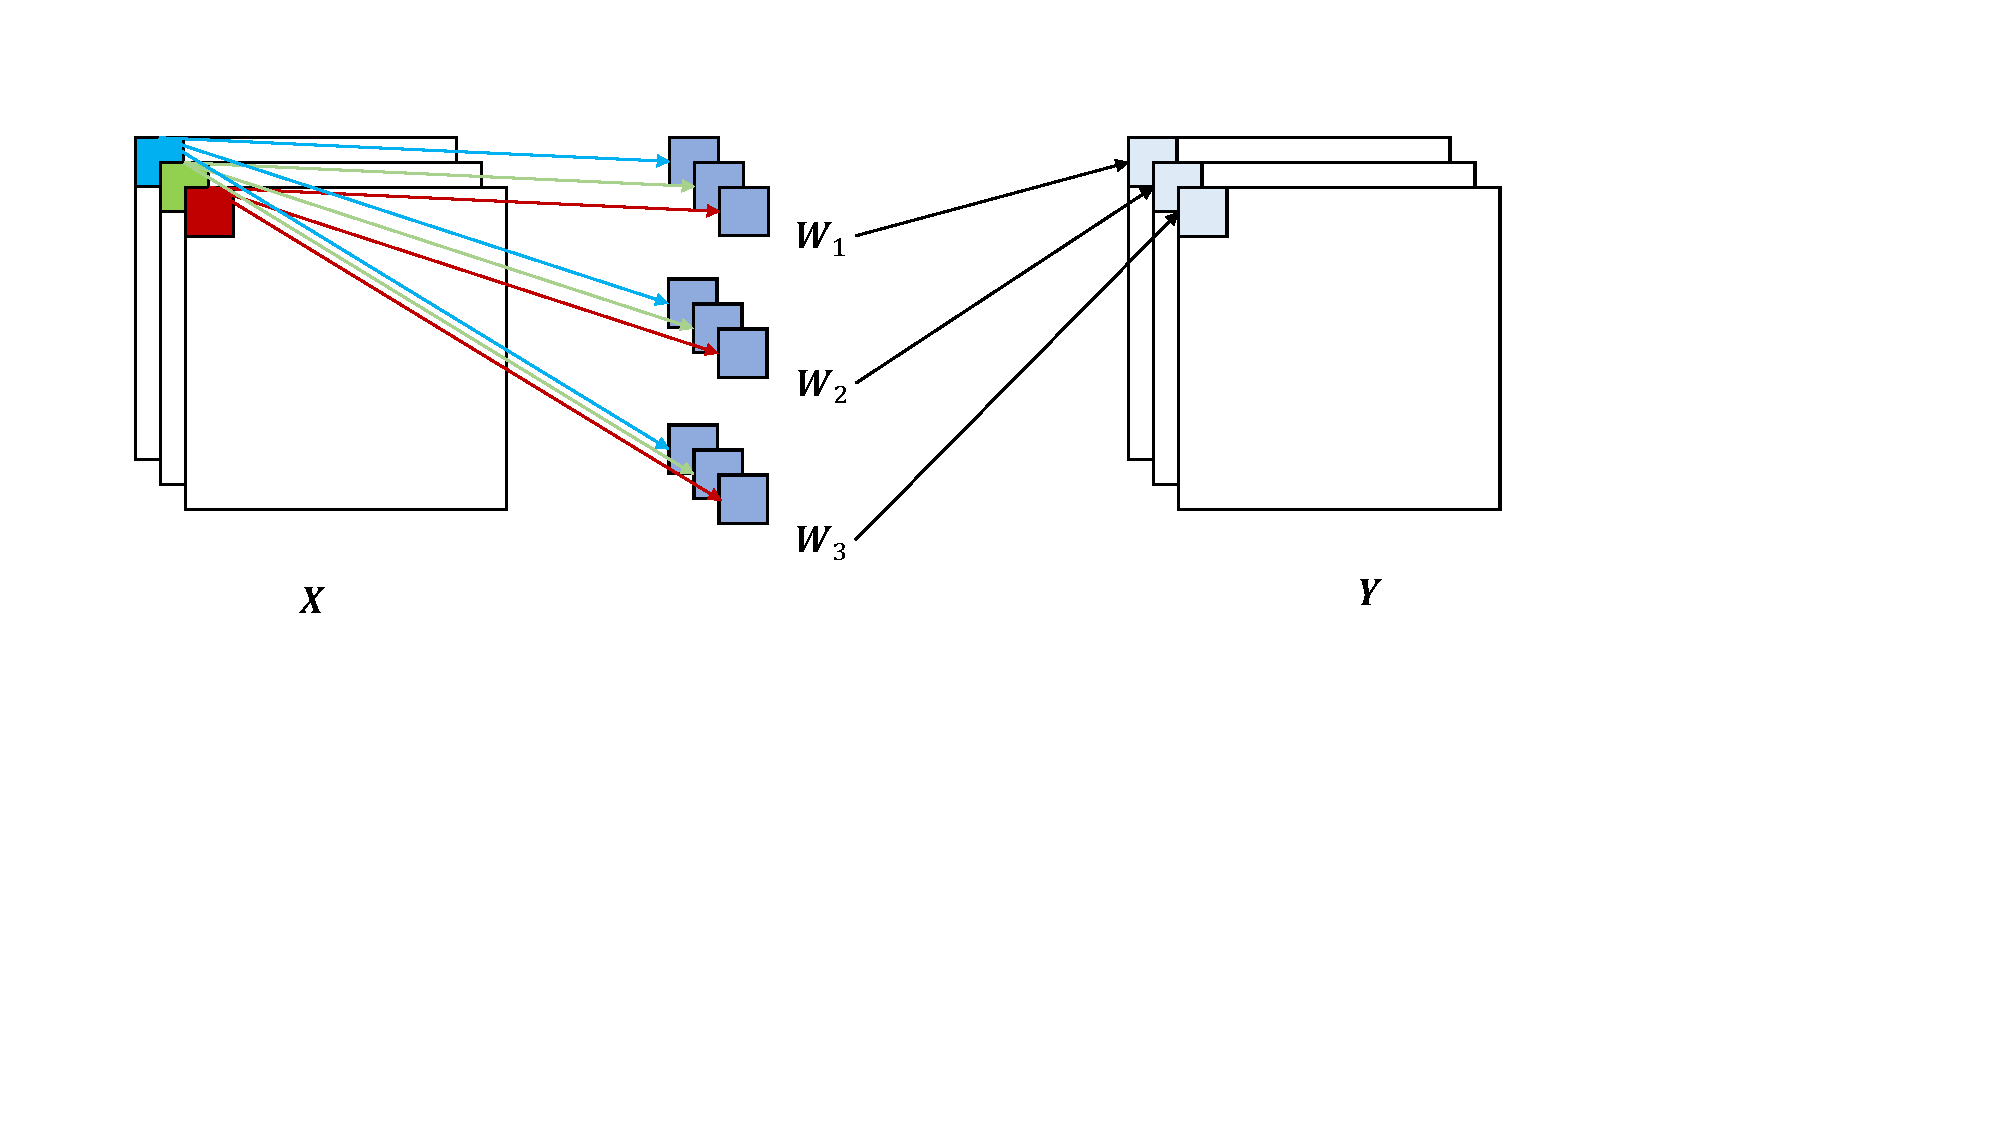
\includegraphics[width=0.6\textwidth]{Figures/1x1convolution}
              \caption{$1\times1$ convolutional layer.}
            \end{figure}
    
    Now we flatten the output $\mathbf{Y}$ to attain a $3\times28\times28$-dimensional vector,
    \begin{align*}
      \mathbf{y}=(y_{1,1,1},y_{1,1,2},\cdots, y_{1,1,28},y_{1,2,1},y_{1,2,2},
      \cdots,y_{1,28,28},y_{2,1,1},y_{2,1,2},\cdots, y_{3,28,28}).
    \end{align*}
    We can also flatten $\mathbf{X}$ to attain a $3\times28\times28$-dimensional vector $\mathbf{x}$.
    \begin{enumerate}
      \item Is the $1\times1$ convolutional operation a linear transformation? If so, Please find the transformation matrix.
      \item Please show that the $1\times1$ convolutional operation is  invertible if and only if the matrix $(\mathbf{w}_1,\mathbf{w}_2,\mathbf{w}_3)$ is invertible.

          \textbf{Hint}: let $A=\left(a_{i j}\right)_{m \times m}$, $B\in\mathbb{R}^{n \times n}$, then the $m n \times m n$ matrix
          \begin{align*}
            \left(\begin{array}{cccc}
            a_{11} B & a_{12} B & \cdots & a_{1 m} B \\
            a_{21} B & a_{22} B & \cdots & a_{2 m} B \\
            \vdots & \vdots & \cdots & \vdots \\
            a_{m 1} B & a_{m 2} B & \cdots & a_{m m} B
            \end{array}\right)
          \end{align*}
          is called the Kronecker product of $A$ and $B$, denoted by $ A \otimes B$. Furthermore, $\operatorname{det}(A \otimes B)=(\operatorname{det}(A))^{n}(\operatorname{det}(B))^{m}$.

      \item Suppose $\mathbf{x}$ is sampled from a standard Gaussian $\mathcal{N}(\mathbf{0},\mathbf{I})$, please find the density function of $\mathbf{y}$ if the $1\times1$ convolutional operation is  invertible.

    \end{enumerate}
    \item \textbf{Pooling layer.} We know that average pooling and overlapping pooling are linear transformations, but not the max pooling.
        \begin{enumerate}
          \item Suppose an average pooling layer has window size $2\times2$ and stride 2, as illustrated in the following picture. The pooling layer takes as inputs the $4\times4 $ matrices.  Please find the transformation matrix of the average pooling layer.
                \begin{figure}[H]
                  \centering
                  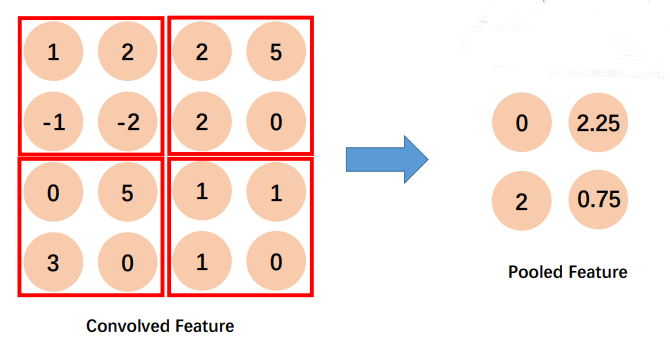
\includegraphics[width=0.6\textwidth]{Figures/pooling.png}
                  \caption{average pooling.}
                \end{figure}

          \item Max pooling is generally not linear transformation. Consider the following example we studied in this course. The max pooling layer has window size $2\times2$ and stride 2, as illustrated in the following picture. The pooling layer takes as inputs the $4\times4 $ matrices. Please find the subgradient of the max pooling operation. Then give an explanation of the ``gradient" we studied in our course.
          \begin{figure}[H]
              \centering
              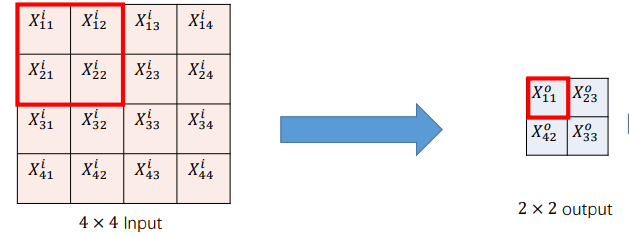
\includegraphics[width=0.6\textwidth]{Figures/max_pooling.png}
              \caption{max pooling.}
            \end{figure}
        \end{enumerate}

\end{enumerate}

\end{exercise}
\begin{solution}

\end{solution}


%%%%%%%%%%%%%%%%%%%%%%%%%%%%%%%%%%%%%%%%%%%%%%%%%%%%%%%%%%%%%%%%

\end{document}
